\subsection{Frame Stack Generation}
\begin{figure}[H]
  \centering
  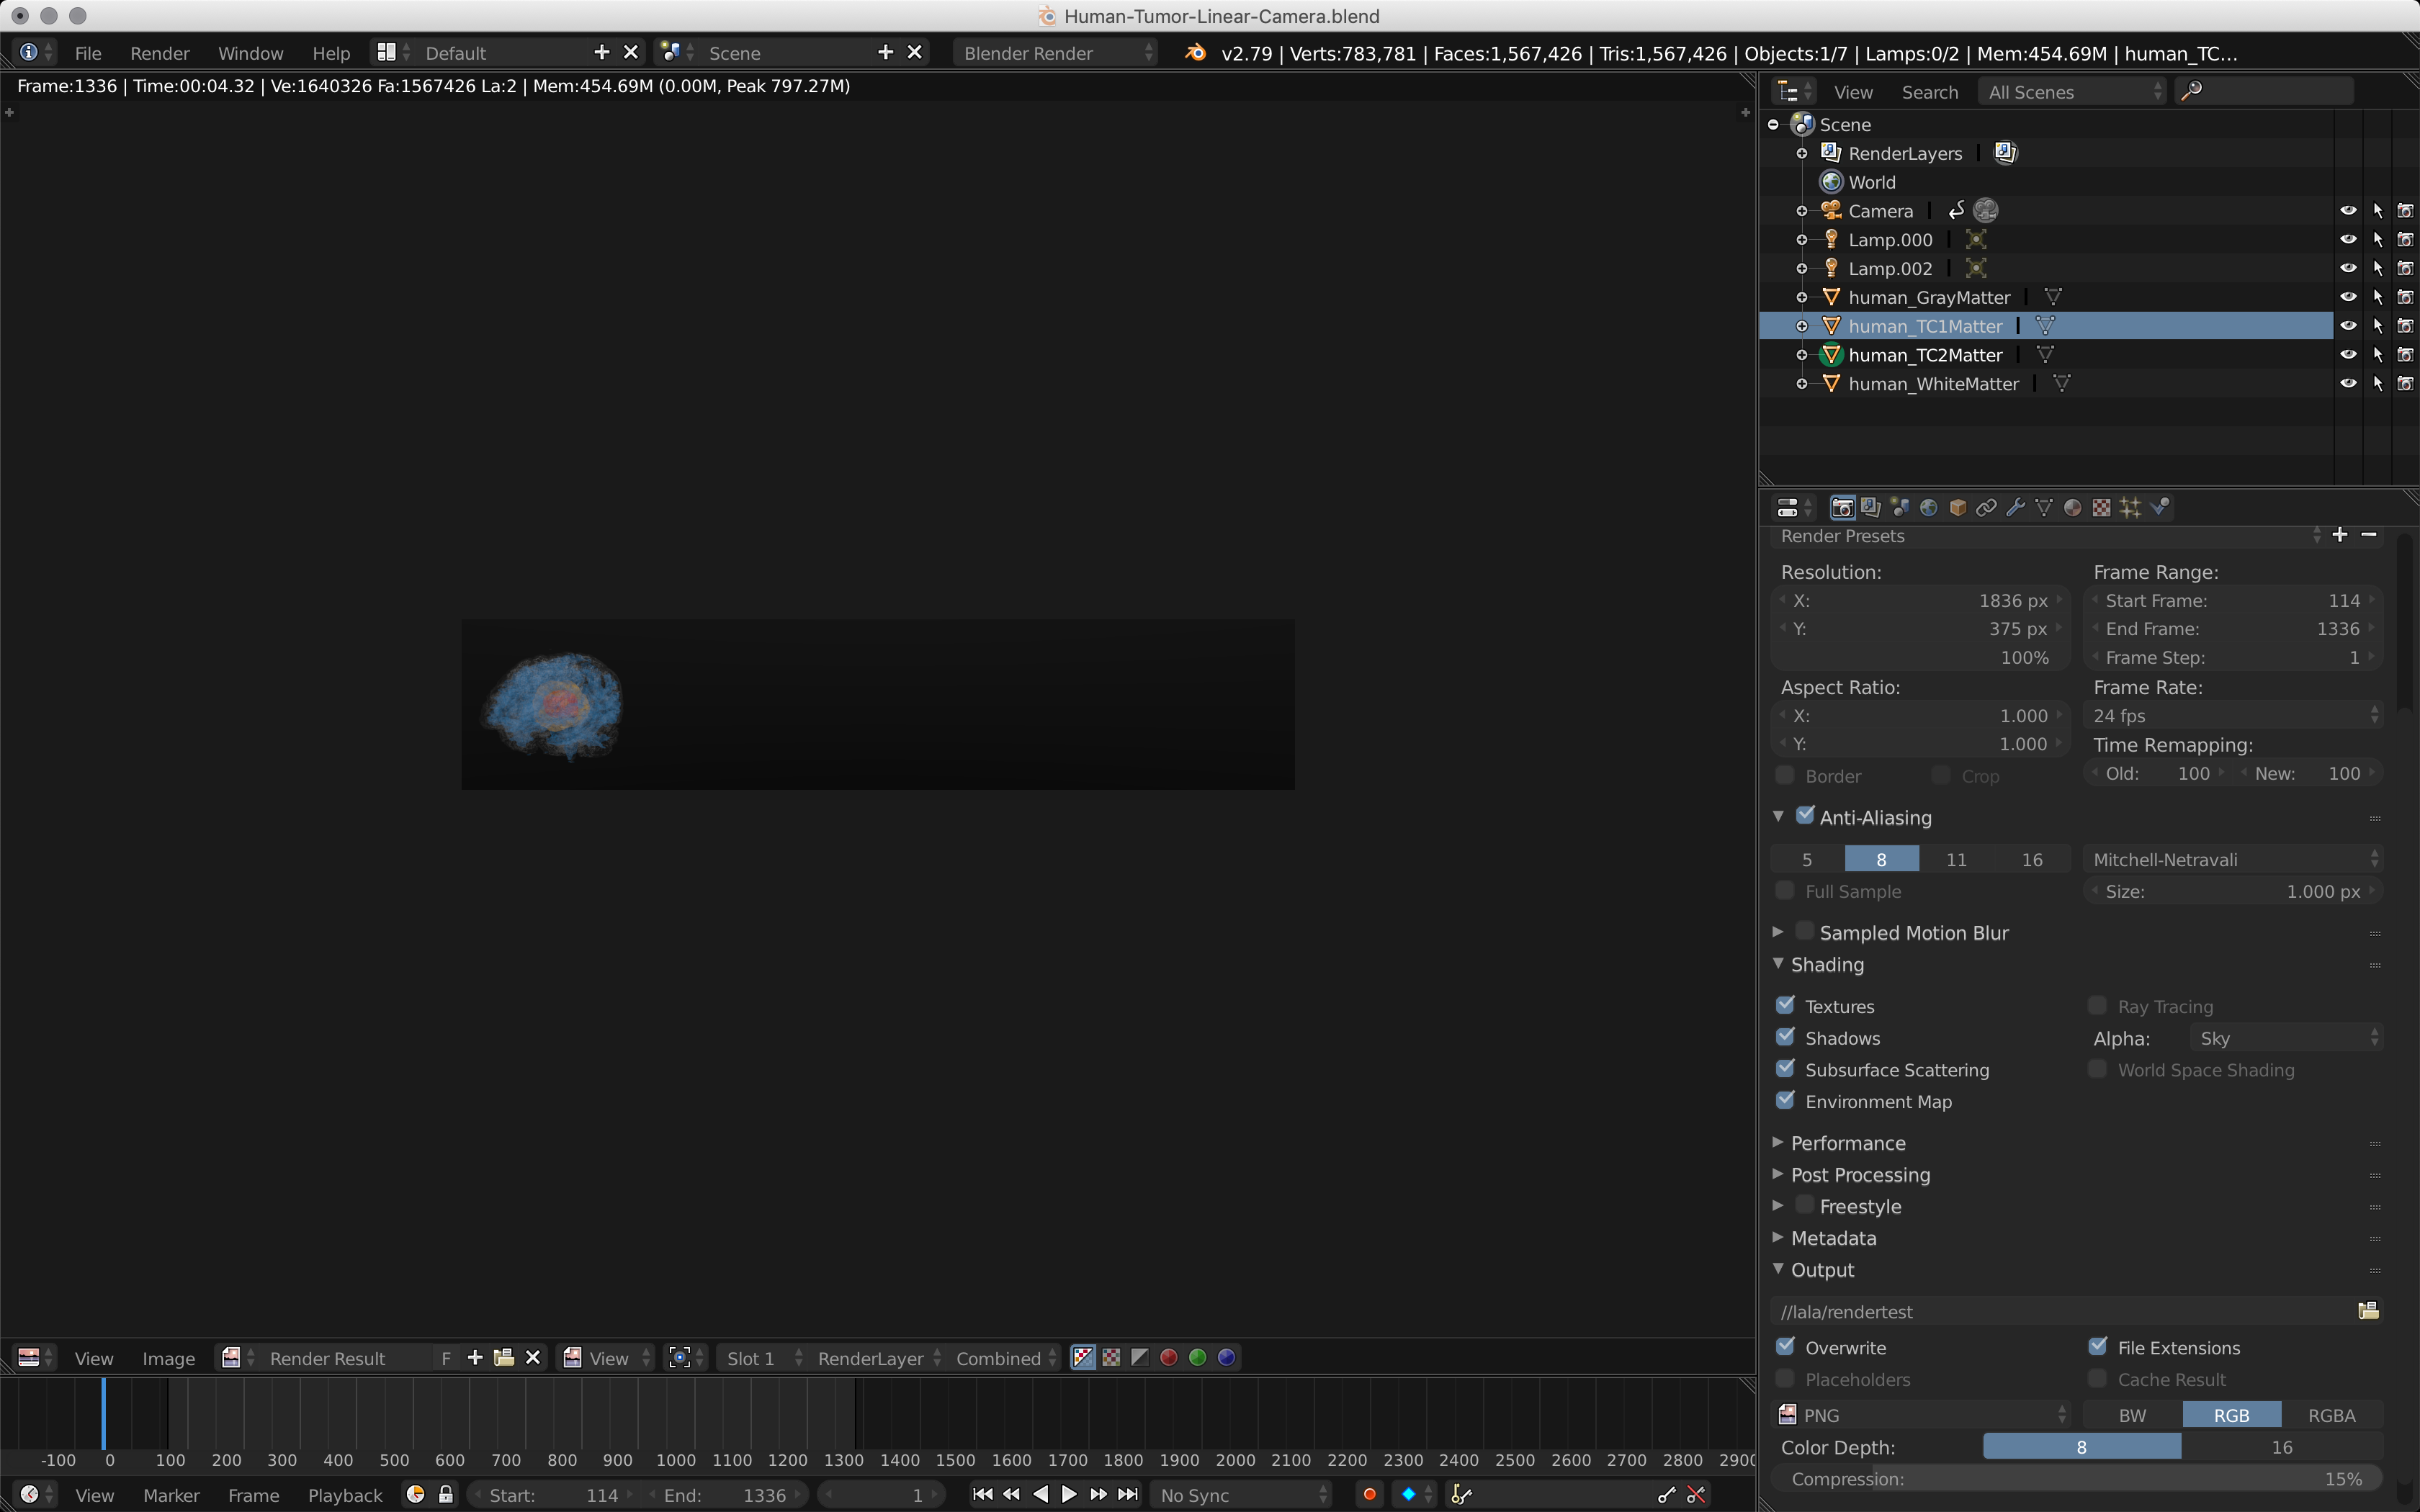
\includegraphics[width=\linewidth]{img/linCam1.png}
  \caption{Blender view of linear camera setup. Image by Marcus A. Gordon.}
  \Description{Blender view of linear camera setup}
\end{figure}

In order to develop our digital hologram, we create a virtual camera setup that mimics the recording behaviour of our holographic printer.  We call this virtual camera setup the `linear camera' as it refers to the linear movement of photographing the three dimensional space from right to left.  This virtually photographed three dimensional space becomes the field of view of the observer of the hologram and holds the dimensionality and depth of the objects in its scene within 1336 angles of view.

The viewing window set for this is 1836px by 375px as shown in Figure 10.

